\chapter*{Affinity 2.0 settings for \gls{bc} vs \gls{ac} match test}
This appendix explain the settings for the Affinity 2.0 for \gls{bc} vs \gls{ac} matching.

\section*{Materials and setup}
To adjust the Affinity 2.0 settings, the following materials are used:
\begin{itemize}
\item Affinity 2.0
\item The Affinity 2.0 control computer
\end{itemize}

\begin{figure}[H]
	\centering
		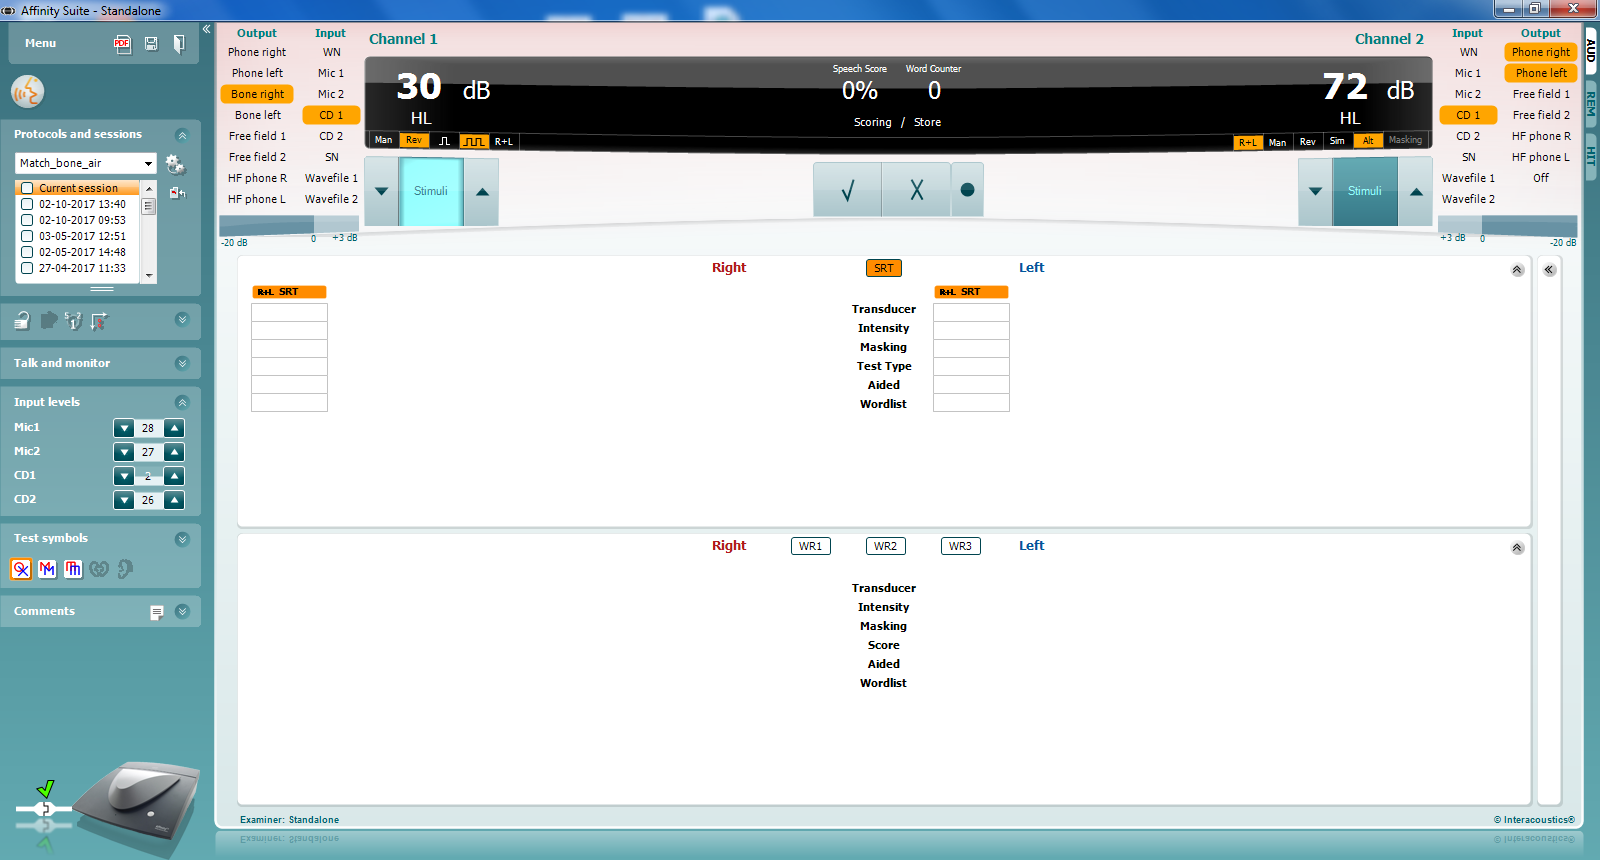
\includegraphics[width=1\textwidth]{match_bone_air}
		\caption{The settings for  \gls{bc} vs \gls{ac} matching}
		\label{fig:apend_match_bone_air}
\end{figure}

\section*{Test procedure}


\begin{enumerate}
\item The materials are set up as in \autoref{fig:appendix:test}.
\item 
\item  
\item  
\item 
\item 
\end{enumerate}

\section*{Results}

\begin{figure}[htbp!]
	\centering
		\includegraphics[width=1\textwidth]{guitar_low_E_neck.pdf}
		\caption{Measurement of the low E note on the neck pickup.}
		\label{fig:appendix:low_E_neck}
\end{figure}

On  \autoref{fig:appendix:low_E_neck} it is seen that the lowest significant frequency is around \SI{80}{\hertz} and the highest significant frequency is around \SI{400}{\hertz}, when playing the low E note on the guitar, using the neck pickup.
